\begin{exercises} 
  \item The instantaneous velocity (in meters per minute) of a moving object is given by the function $v$ as pictured in Figure~\ref{F:4.4.Ez2}.  Assume that on the interval $0 \le t \le 4$, $v(t)$ is given by $v(t) = -\frac{1}{4}t^3 + \frac{3}{2}t^2 + 1$, and that on every other interval $v$ is piecewise linear, as shown.
  \begin{figure}[h]
\begin{center}
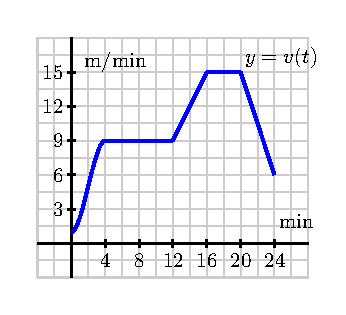
\includegraphics{figures/4_4_Ez2.eps}
\caption{The velocity function of a moving body.} \label{F:4.4.Ez2}
\end{center}
\end{figure} 
  \ba
  	\item Determine the exact distance traveled by the object on the time interval $0 \le t \le 4$.
	\item What is the object's average velocity on $[12,24]$?
	\item At what time is the object's acceleration greatest?
	\item Suppose that the velocity of the object is increased by a constant value $c$ for all values of $t$.  What value of $c$ will make the object's total distance traveled on $[12,24]$ be 210 meters?
  \ea
    \item A function $f$ is given piecewise by the formula
  $$f(x) = \left\{ 
  	\begin{array}{lr}
	-x^2 + 2x + 1, & \ \mbox{if} \ 0 \le x < 2 \\
	-x + 3, & \ \mbox{if} \ 2 \le x < 3 \\
	x^2 - 8x + 15, & \ \mbox{if} \ 3 \le x \le 5
	\end{array}
	\right.
  $$
  \ba
  	\item Determine the exact value of the net signed area enclosed by $f$ and the $x$-axis on the interval $[2,5]$.
	\item Compute the exact average value of $f$ on $[0,5]$.
	\item Find a formula for a function $g$ on $5 \le x \le 7$ so that if we extend the above definition of $f$ so that $f(x) = g(x)$ if $5 \le x \le 7$, it follows that $\int_0^7 f(x) \, dx = 0.$
  \ea

  \item When an aircraft attempts to climb as rapidly as
possible, its climb rate (in feet per minute) decreases as altitude
increases, because the air is less dense at higher altitudes.
Given below is a table showing performance data for a certain
single engine aircraft, giving its climb rate at various altitudes, where  $c(h)$ denotes the climb rate of the airplane at an altitude $h$.

\begin{center}
  \begin{tabular}{|c||c|c|c|c|c|c|c|c|c|c|c|}
    \hline
    $h$ (feet)&0&1000&2000&3000&4000&5000&6000&7000&8000&9000&10,000\\
    \hline
    $c$ (ft/min)&925&875&830&780&730&685&635&585&535&490&440\\
    \hline
  \end{tabular}
\end{center}

 Let a new function called $m(h)$ measure
the number of minutes required for a plane at altitude $h$ to climb the
next foot of altitude.
\ba
	\item Determine a similar table of values for $m(h)$ and explain how it is related to the table above.  Be sure to explain the units.

	\item Give a careful interpretation of a function whose derivative
is $m(h)$.  Describe what the input is and what the output is.  Also,
explain in plain English what the function tells us.

	\item Determine a definite integral whose value tells us exactly the number of minutes required for the airplane to ascend to
10,000 feet of altitude.  Clearly explain why the value of this integral has the required meaning.

	\item Use the Riemann sum $M_5$ to estimate the value of the integral you found in (c).  Include units on your result.
\ea

  \item In Chapter~\ref{C:1}, we showed that for an object moving along a straight line with position function $s(t)$, the object's ``average velocity on the interval $[a,b]$'' is given by 
  $$\displaystyle AV_{[a,b]} =  \frac{s(b)-s(a)}{b-a}.$$
	
	More recently in Chapter~\ref{C:4}, we found that for an object moving along a straight line  with velocity function $v(t)$, the object's ``average value of its velocity function on $[a,b]$'' is 
	$$\displaystyle v_{\mbox{\tiny{AVG}}[a,b]}  = \frac{1}{b-a} \int_a^b v(t) \, dt.$$
	
Are the ``average velocity on the interval $[a,b]$'' and the ``average value of the velocity function on $[a,b]$'' the same thing?  Why or why not?  Explain.

\end{exercises}
\afterexercises
